\documentclass[border=1mm]{standalone}
\usepackage{amsfonts, tikz, tikz-layers}
\usetikzlibrary{fadings, quotes, shapes, calc, decorations.markings}
\usetikzlibrary{patterns}
\usetikzlibrary{shadows.blur}
\usetikzlibrary{shapes, shapes.geometric, positioning, arrows, arrows.meta}
\usetikzlibrary{backgrounds}

\definecolor{fblue}{HTML}{9accff}
\definecolor{dblue}{HTML}{386aff}

\begin{document}
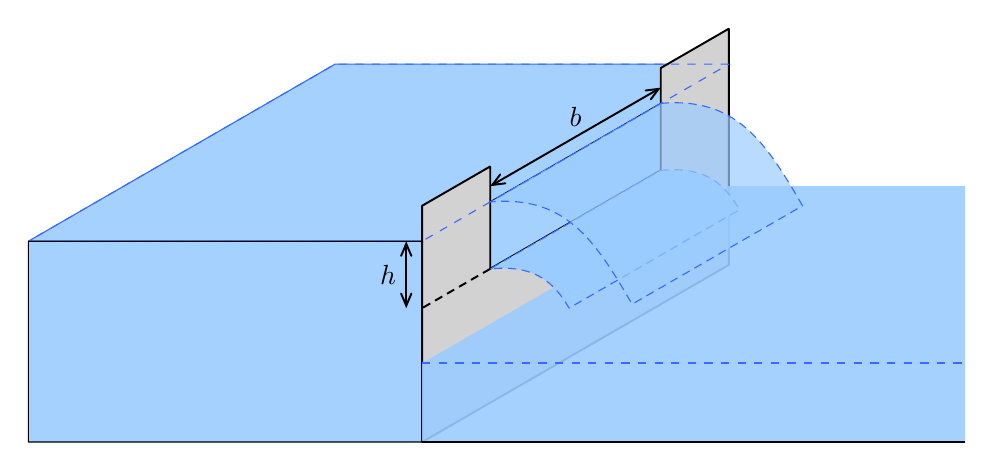
\begin{tikzpicture}[line join=bevel, line width=.7pt]

\begin{scope}[]
\draw[fill=gray!35] (0,3)-- coordinate[pos=1] (p1) ++(0,-3)--++(30:4.5)--coordinate[pos=.85] (p2)++(0,3)--++(180+30:1)--++(0,-1.3)--++(180+30:2.5)--++(0,1.3)--cycle;
\end{scope}

\begin{scope}[on background layer]
\draw[dblue,fill=fblue,line join=bevel,fill opacity=.9] (p2)--++(-5,0)--coordinate[pos=1](p3)++(180+30:4.5)--++(5,0)--cycle;
\draw[fill=fblue,line join=bevel,fill opacity=.9] (p3)--(p3|-p1)--(p1)--++(30:4.5)--(p2)--coordinate[pos=.222](z1) coordinate[pos=.778](z2)++(180+30:4.5)--cycle;
\end{scope}

\coordinate (p5) at ([yshift=1cm]p1);
\fill[fblue,fill opacity=.9] (p5)--++(30:4.5)--coordinate[pos=1] (p4)++(3,0)--(p4|-p1)--(p1)--cycle;
\draw[dblue,dashed] (p5)--(p4|-p5);
\draw (p1)--(p1-|p4);

\begin{scope}[on above layer]
\draw[densely dashed,dblue,fill=fblue,line join=bevel,fill opacity=1] ([yshift=-.85cm]z1) to[out=5, in =120, looseness=1.1] ++(1,-.5)--++(180+30:2.5) to[in=5, out =120, looseness=1.1] ([yshift=-.85cm]z2)--cycle;
\draw[densely dashed,dblue,fill=fblue,line join=bevel, fill opacity=.7] (z1) to[out=5, in =120, looseness=1.1] ++(1.8,-1.3)--++(180+30:2.5) to[in=5, out =120, looseness=1.1] (z2)--cycle;
\end{scope}

\draw[dblue,line join=bevel, dashed, line width=.4pt] (p2)--++(-5,0)--coordinate[pos=1](p3)++(180+30:4.5)--++(5,0)--cycle;
\draw[line join=bevel,line width=.5pt] (p3)--++(5,0);

\draw[angle 45-angle 45] ([yshift=.2cm]z1)--node[above]{$b$}([yshift=.2cm]z2);
\draw[black,densely dashed] ([yshift=-.85cm]z2)--coordinate[pos=1](z3)++(180+30:1);
\draw[angle 45-angle 45] ([xshift=-2mm]z3)--node[left]{$h$}++(0,.85);


\end{tikzpicture}

\end{document}
